% chap3.tex
%

\mychapter{Structured and Unstructured Data for Factoid Question Answering}
\label{chapter:factoid}

\noindent

There are multiple ways to marry unstructured and structured data for joint question answering: convert structured data to unstructured format or vice versa, convert all data to certain intermediate representation or to leave them as is and link the data sources.
In my thesis I focus on two approaches: relation extraction for knowledge base completion, and semantic annotation of text for hybrid question answering.

\section{Relation Extraction for Knowledge Base Completion}
\label{sec:relation_extraction}

The information on the web is stored in multiple different forms, such as natural language statements, tables and infoboxes, images \etc.
In this work I focus on yet another source of information: question-answer pairs.
Community question answering archives contain hundreds of millions of question and corresponding answers.
Information expressed in these pairs might be hard to extract or not exist at all in other formats.

\subsection{Relation extraction from Question-Answer pairs}
\label{subsec:cqa_relextract}

CQA websites, such as Yahoo! Answers\footnote{http://answers.yahoo.com/}, Answers.com\footnote{http://www.answers.com}, Quora\footnote{http://quora.com} \etc, has gained a lot of popularity in the recent years, and their archives store hundreds of millions of user questions along with answers provided by the community.
Many users' information needs are not unique and arise again and again, which makes it possible to reuse the information to answers new questions \cite{Shtok:2012:LPA:2187836.2187939}.
This idea makes CQA data attractive for knowledge base population.
Although some of the facts mentioned in QnA pairs can also be found in some other text documents, another part might be unique (\eg in Clueweb\footnote{http://www.lemurproject.org/clueweb12/} about 10\% of entity pairs with existing Freebase relations mentioned in Yahoo! Answers documents cannot be found in other documents \cite{savenkov2015relation}).
Existing relation extraction techniques face some challenges when applied to CQA data, \ie they typically consider sentences independently and ignore the discourse of a QnA pair text.
However, frequently, it is impossible to understand the answer without knowing the question.
For example, sometimes users simply give the answer to the question without stating it in a narrative sentence (\eg ``\emph{What does "xoxo" stand for? Hugs and kisses.}``), or the provided answer might contain ellipsis, \ie some important information is omitted (\eg ``\emph{What's the capital city of Bolivia? Sucre is the legal capital, though the government sits in La Paz}``).

In this thesis we propose a novel model for relation extraction from CQA data, that uses discourse of a QnA pair to extract facts between entities mentioned in question and entities mentioned in answer sentences.
The conducted experiments confirm that many of such facts cannot be extracted by existing sentence-based techniques and thus it is beneficial to combine their outputs with the output of our model. 

Let us define the problem more formally.
We target the problem of relation extraction from QnA data, which is a collection of $(q, a)$ pairs, where $q$ is a question text (can contain multiple sentences) and $a$ is the corresponding answer text (can also contain multiple sentences).
By relation instance $r$ we mean an ordered binary relation between $subject$ and $object$ entities, which is commonly represented as $[subject, predicate, object]$ triple.
For example, the fact that Brad Pitt married Angelina Jolie can be represented as [Brad Pitt, married\_to, Angelina Jolie].
In this work we use Freebase, an open schema-based KB, where all entities and predicates come from the fixed alphabets $E$ and $P$ correspondingly.
% The relation extraction problem can be formulated as a multiple instance multi-label classification problem \cite{Surdeanu:2012:MML:2390948.2391003}.
Let $e_1$ and $e_2$ be entities that are mentioned together in a text (\eg in a sentence, or $e_1$ in a question and $e_2$ in the corresponding answer), we will call such an entity pair with the corresponding context a mention.
The same pair of entities can be mentioned multiple times within the corpus, and for all mentions $i=1,...,n$ the goal is to predict the expressed predicate ($z_i \in P$) or to say that none applies ($z_i = \emptyset$).
Individual mention predictions $z_1, ..., z_n$ are combined to infer a set of relations $\mathbf{y}=\{y_i \in P\}$ between the entities $e_1$ and $e_2$.

\begin{figure}[h]
\centering
\begin{tikzpicture}
\tikzstyle{main}=[circle, minimum size = 8mm, thick, draw =black!80, node distance = 14mm]
\tikzstyle{mainnob}=[circle, minimum size = 8mm, thick, draw =white!100, node distance = 14mm]
\tikzstyle{connect}=[-latex, thick]
\tikzstyle{box}=[rectangle, draw=black!100]
\node[main, fill = white!100] (y) [label=center:$y$] { };
\node[rectangle, inner sep=-1mm, fit=(y),label=below right:$P$] {};
\node[rectangle, inner sep=4mm, fit=(y),draw=black!100] {};
\node[main, fill = white!100] (z) [below=of y,label=center:$z$] { };
%\node[rectangle, inner sep=-1mm, fit=(z),label=below right:$P$] {};
%\node[rectangle, inner sep=4mm, fit=(z),draw=black!100] {};
\node[main, fill = black!10] (x) [below=of z,label=center:$\mathbf{x}$] { }; 
\node[main, fill = black!10] (t) [right=of z,label=center:$\mathbf{x_t}$] { };
\node[mainnob, fill = white!100] (wt) [right=of y,label=center:$\mathbf{w_t}$] { };
\node[mainnob, fill = white!100] (wx) [left=of y,label=center:$\mathbf{w_x}$] { };
\node[rectangle, inner sep=-1mm, fit=(z)(x)(t),label=below right:$|Q|$, yshift=-1mm] {};
\node[rectangle, inner sep=6.5mm, fit=(z)(x)(t),draw=black!100] {};

\node[rectangle, inner sep=-1mm, fit=(z)(x),label=below right:$M$,yshift=-12mm] {};
\node[rectangle, inner sep=5.0mm, fit=(z)(x),draw=black!100] {};

\node[rectangle, inner sep=-1mm, fit=(x)(z)(y),label=below right:$N$,yshift=-30mm,xshift=4.5mm] {};
\node[rectangle, inner sep=9mm, fit=(x)(z)(y),draw=black!100, yshift=-3mm] {};

\path (wx) edge [connect] (z)
(x) edge [connect] (z)
(z) edge [connect] (y)
(wt) edge [connect] (z)
(t) edge [connect] (z);
\end{tikzpicture}
\vspace{-15mm}
\caption{QnA-based relation extraction model plate diagram.
$N$ - number of different entity pairs, $M$ - number of mentions of an entity pair, $|Q|$ - number of questions where an entity pair is mentioned, $\mathbf{x}$ and $\mathbf{x_t}$ - mention-based and question-based features, $\mathbf{w}$ and $\mathbf{w_t}$ - corresponding feature weights, latent variables $z$ - relation expressed in an entity pair mention, latent variables $y$ - relations between entity pair}
\label{fig:qna_relextract:graphmodel}
\end{figure}

Our models for relation extraction from QnA data incorporates the topic of the question and can be represented as a graphical model (Figure \ref{fig:qna_relextract:graphmodel}).
Each mention of a pair of entities is represented with a set of mention-based features $x$ and question-based features $x_t$.
A multinomial latent variable $z$ represents a relation (or none) expressed in the mention and depends on the features and a set of weights $w_x$ for mention-based and $w_t$ for question-based features:
$$\hat{z}=\argmax{z \in P \cup \emptyset} p(z|x, x_t, w_x, w_t)$$.
To estimate this variable we use L2-regularized multinomial logistic regression model, trained using the distant supervision approach for relation extraction \cite{MintzBSJ09}, in which mentions of entity pairs related in Freebase are treated as positive instances for the corresponding predicates, and negative examples are sampled from mentions of entity pairs which are not related by any of the predicates of interest.
Finally, to predict a set of possible relations $\mathbf{y}$ between the pair of entities we take logical OR of individual mention variables $\mathbf{z}$, \ie $y_p = \lor_{i=1}^M [z_i = p, p \in P]$, where M is the number of mentions of this pair of entities.

\subsubsection{Sentence-based baseline model}

Existing sentence-based relation extraction models can be applied to individual sentences of a QnA pair and will work well for complete statements, \eg ``Who did Brad Pitt marry? Brad Pitt and Angelina Jolie married at secret ceremony''.
In sentence-based scenario, when the set of question-based features is empty, the above model corresponds to the Mintz++ baseline described in \cite{Surdeanu:2012:MML:2390948.2391003}, which was shown to be superior to the original model of \cite{MintzBSJ09}, is easier to train than some other state of the art distant supervision models and produces comparable results.

\subsubsection{Sentence-based model with question features}

\begin{table*}[tbh]
\centering
\caption{Examples of features used for relation extraction for ``\emph{When was Mariah Carey born? Mariah Carey was born 27 March 1970}''}
\vspace{-2mm}
\label{table:qna_relextract:features}
\begin{tabular}{|p{8cm}|p{8cm}|}
\hline
\multicolumn{2}{|c|}{Sentence-based model}\\
\hline
Dependency path between entities & [PERSON]$\rightarrow$nsubjpass(born)tmod$\leftarrow$[DATE]\\
Surface pattern & [PERSON] be/VBD born/VBN [DATE]\\
\hline
\hline
\multicolumn{2}{|c|}{Question features for sentence-based model}\\
\hline
Question template & when [PERSON] born\\
Dependecy path from a verb to the question word & (when)$\rightarrow$advmod(born)\\
Question word + dependency tree root & when+born\\
\hline
\hline
\multicolumn{2}{|c|}{QnA-based model}\\
\hline
Question template + answer entity type & Q: when [PERSON] born A:[DATE]\\
Dependency path from question word to entity & Q:(when)$\rightarrow$advmod(born)nsubj$\leftarrow$[PERSON]\\
and answer entity to the answer tree root & A: (born)tmod$\leftarrow$[DATE]\\
Question word, dependency root and answer pattern & Q: when+born A:born [DATE]\\
\hline
\end{tabular}
\end{table*}

In many cases an answer statement is hard to interpret correctly without knowing the corresponding question.
To give the baseline model some knowledge about the question, we include question features (Table \ref{table:qna_relextract:features}), which are based on dependency tree and surface patterns of a question sentence. 
This information can help the model to account for the question topic and improve predictions in some ambiguous situations.

\subsubsection{QnA-based model}
The QnA model for relation extraction is inspired by the observation, that often an answer sentence do not mention one of the entities at all, \eg, ``\textit{When was Isaac Newton born? December 25, 1642 Woolsthorpe, England}''.
To tackle this situation we make the following assumption about the discourse of a QnA pair: an entity mentioned in a question is related to entities in the corresponding answer and the context of both mentions can be used to infer the relation predicate.
Our QnA-based relation extraction model takes an entity from a question sentence and entity from the answer as a candidate relation mention, represents it with a set features (Table \ref{table:qna_relextract:features}) and predicts a possible relation between them similar to sentence-based models.
The features are conjunctions of various dependency tree and surface patterns of question and answer sentences, designed to capture their topics and relation.

\subsubsection{Experiments}

For experiments we used 2 publicly available CQA datasets: Yahoo! Answers WebScope dataset\footnote{http://webscope.sandbox.yahoo.com/catalog.php?datatype=l} and a crawl of WikiAnswers\footnote{http://wiki.answers.com/} collected by \cite{Fader:2014:OQA:2623330.2623677}.
The Yahoo! Answers dataset contains 4,483,032 questions (3,894,644 in English) with the corresponding answers collected on 10/25/2007.
The crawl of WikiAnswers has 30,370,994 question clusters, tagged by WikiAnswers users as paraphrases, and only 3,386,256 them have answers.
From these clusters we used all possible pairs of questions and corresponding answers (19,629,443 pairs in total).

\begin{table*}[ht]
\centering
\caption{Yahoo! Answers and WikiAnswers datasets statistics}
\vspace{-2mm}
\label{table:qna_relextract:cqastats}
\begin{tabular}{|p{12.5cm}||p{1.2cm}|p{1.2cm}|} \hline
& Y!A & WA\\
\hline
Number of QnA pairs & 3.8M & 19.6M \\
Average question length (in chars) & 56.67 & 47.03 \\
Average answer length (in chars) & 335.82 & 24.24 \\
% Number of resolved entities per QnA pair & 3.57 & 3.23 \\
Percent of QnA pairs with answers that do not have any verbs & 8.8\% & 18.9\% \\
Percent of QnA pairs with at least one pair of entities related in Freebase & 11.7\% & 27.5\% \\
Percent of relations between entity pairs in question sentences only & 1.6 \% & 3.1\% \\
Percent of relations between entity pairs in question and answer sentences only & 28.1\% & 46.4\% \\
Percent of relations between entity pairs in answer sentences only & 38.6\%& 12.0\%\\
\hline
\end{tabular}
\end{table*}

For each QnA pair we applied tokenization, sentence detection, named entity tagger, parsing and coreference resolution from Stanford CoreNLP \cite{manning-EtAl:2014:P14-5}.
Our cascade entity linking approach is similar to \cite{chang2011stanford} and considered all noun phrase and named entity mentions as candidates.
First all named entity mentions are looked up in Freebase names and aliases dictionary.
The next two stages attempt to match mention text with dictionary of English Wikipedia concepts \cite{spitkovsky2012cross} and its normalized version.
Finally for named entity mentions we try spelling correction using Freebase entity names dictionary.
We didn't disambiguate entities and instead took top-5 ids for each coreference cluster (using the $p(entity|phrase)$ score from the dictionary or number of existing Freebase triples).
All pairs of entities (or entity and date) in a QnA pair that are directly related\footnote{We also consider some paths that come through a mediator node, \eg  /people/person/spouse\_s./people/marriage/spouse} in Freebase were annotated with the corresponding relations.

Table \ref{table:qna_relextract:cqastats} gives some statistics on the datasets used in this work.
The analysis of answers that do not have any verbs show that $\sim$8.8\% of all QnA pairs do not state the predicate in the answer text.
The percentage is higher for WikiAnswers, which has shorter answers on average.
Unfortunately, for many QnA pairs we were unable to find relations between the mentioned entities (for many of them no or few entities were resolved to Freebase).
Among those QnA pairs, where some relation was annotated, we looked at the location of related entities.
In Yahoo! Answers dataset 38.6\% (12.0\% for WikiAnswers) of related entities are mentioned in answer sentences and can potentially be extracted by sentence-based model, and 28.1\% (46.4\% for WikiAnswers) between entities mentioned in question and answer sentences, which are not available to the baseline model and our goal is to extract some of them.

For our experiments we use a subset of 29 Freebase predicates that have enough unique instances annotated in our corpus, \eg date of birth, profession, nationality, education institution, date of death, disease symptoms and treatments, book author, artist album, \etc
We train and test the models on each dataset separately.
Each corpus is randomly split for training (75\%) and testing (25\%).
Knowledge base facts are also split into training and testing sets (50\% each).
QnA and sentence-based models predict labels for each entity pair mention, and we aggregate mention predictions by taking the maximum score for each predicate.
We do the same aggregation to produce a combination of QnA- and sentence-based models, \ie, all extractions produced by the models are combined and if there are multiple extractions of the same fact we take the maximum score as the final confidence.
The precision and recall of extractions are evaluated on a test set of Freebase triples, \ie an extracted triple is considered correct if it belongs to the test set of Freebase triples, which are not used for training (triples used for training are simply ignored).
Note, that this only provides a lower bound on the model performance as some of the predicted facts can be correct and simply missing in Freebase.

Figure \ref{fig:qna_relextract:pr_curve} shows Precision-Recall curves for QnA-based and sentence-based baseline models and some numeric results are given in Table \ref{table:qna_relextract:results}.
As 100\% recall we took all pairs of entities that can be extracted by either model.
It is important to note, that since some entity pairs occur exclusively inside the answer sentences and some in pairs of question and answer sentences, none of the individual models is capable of achieving 100\% recall, and maximum possible recalls for QnA- and sentence-based models are different.

\begin{figure}[h!]
\centering
\vspace{-2mm}
\begin{subfigure}[h]{0.45\textwidth}
	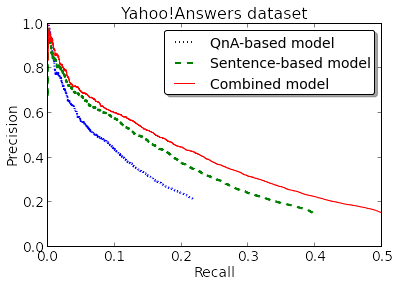
\includegraphics[width=0.99\textwidth]{img/qa_vs_sent_ya}
	\vspace{-1mm}
    \label{figure:pr:ya}
\end{subfigure}
\begin{subfigure}[h]{0.45\textwidth}
	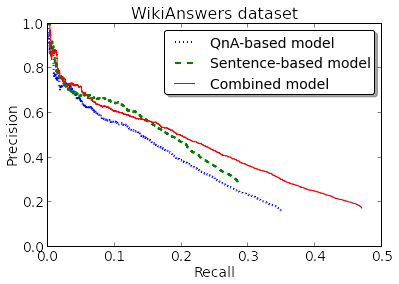
\includegraphics[width=0.99\textwidth]{img/qa_vs_sent_wa}
	\vspace{-1mm}
    \label{figure:pr:wa}
\end{subfigure}
\begin{subfigure}[h]{0.45\textwidth}
	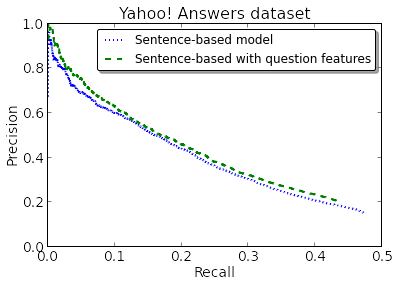
\includegraphics[width=0.99\textwidth]{img/noqf_vs_qf}
	\vspace{-1mm}
	\label{figure:pr:noqf_vs_qf}
\end{subfigure}
\vspace{-1mm}
\caption{Precision-Recall curves for QnA-based vs sentence-based models and sentence-based model with and without question features}
\label{fig:qna_relextract:pr_curve}
\end{figure}

\begin{table*}[tbh]
\centering
\caption{Extraction results for QnA- and sentence-based models on both datasets}
\vspace{-2mm}
\label{table:qna_relextract:results}
\begin{tabular}{|p{6.6cm}||p{0.9cm}|p{1.4cm}|p{1.6cm}||p{0.9cm}|p{1.4cm}|p{1.6cm}|}
\hline
& \multicolumn{3}{|c||}{Yahoo! Answers} & \multicolumn{3}{|c|}{WikiAnswers}\\
\cline{2-7}
& QnA & Sentence & Combined & QnA & Sentence & Combined\\
\hline
F-1 score & 0.219 & 0.276 & 0.310 & 0.277 & 0.297 & 0.332\\
Number of correct extractions & 3229 & 5900 & 7428 & 2804 & 2288 & 3779 \\
Correct triples not extracted by other model & 20.5\% & 56.5\% & - & 39.4\% & 25.8\% & - \\
\hline
\end{tabular}
\end{table*}

Results demonstrate that from 20.5\% to 39.4\% of correct triples extracted by the QnA-based model are not extracted by the baseline model, and the combination of both models is able to achieve higher precision and recall.
Unfortunately, comparison of sentence-based model with and without question-based features (Figure \ref{fig:qna_relextract:pr_curve}) didn't show a significant difference.

\subsubsection{Analysis}

To get an idea of typical problems of QnA-based model we sampled and manually judged extracted high confidence examples that are not present in Freebase (and thus are considered incorrect for precision-recall analysis).

The major reason (40\%) of false positive extractions is errors in entity linking.
For example: ``\emph{Who is Tim O'Brien? He was born in Austin on October 1, 1946}''.
The model was able to correctly extract [Tim O'Brien, date\_of\_birth, October 1, 1946], however Tim O'Brien was linked to a wrong person.
In a number of cases (16\%) our discourse model turns out to be too simple and fails for answers, that mention numerous additional information, \eg ``\emph{How old is Madonna really? ...Cher was born on 20 May 1946 which makes her older that Madonna...}''.
A possible solution would be to either restrict QnA-based model to cases when no additional information is present or design a better discourse model with deeper analysis of the answer sentence and its predicates and arguments.
Some mistakes are due to distant supervision errors, for example for the music.composition.composer predicate our model extracts singers as well as composers (which are in many cases the same).

Of course, there are a number of cases, when our extractions are indeed correct, but are either missing (33\%) or contradicting with Freebase (8\%).
An example of an extracted fact, that is missing in Freebase is ``\emph{Who is Wole Soyinka? He studied at the University College, Ibadan(1952-1954) and the University of Leeds (1954-1957)}'', and [Wole Soyinka, institution, University of Leeds] is currently not present in Freebase.
Contradictions with Freebase occur because of different precision levels (``pianist'' vs ``jazz pianist'', city vs county, \etc), different calendars used for dates or ``incorrect'' information provided by the user.
An example, when existing and extracted relation instance are different in precision is:``\emph{Who is Edward Van Vleck? Edward Van Vleck was a mathematician born in Middletown, Connecticut}'' we extract [Edward Van Vleck, place\_of\_birth, Middletown], however the Freebase currently has USA as his place of birth.

The problem of ``incorrect'' information provided in the answer is very interesting and worth special attention.
It has been studied in CQA research, \eg \cite{shah2010evaluating}, and an example of such QnA pair is: ``\emph{Who is Chandrababu Naidu? Nara Chandra Babu Naidu (born April 20, 1951)}''.
Other authoritative resources on the Web give April 20, 1950 as Chandrababu Naidu's date of birth.
This raises a question of trust to the provided answer and expertise of the answerer.
Many questions on CQA websites belong to the medical domain, \eg people asking advices on different health related topics.
How much we can trust the answers provided to extract them into the knowledge base?
We leave this question to the future work.

Finally, we have seen that only a small fraction of available QnA pairs were annotated with existing Freebase relations, which shows a possible limitation of Freebase schema.
A promising direction for future work is automatic extraction of new predicates, which users are interested in and which can be useful to answer more future questions.

\subsubsection{Conclusion}

In this section we described a model for relation extraction from QnA data, which is capable of predicting relations between entities mentioned in question and answer sentences.
We conducted experiments on 2 publicly available CQA datasets and showed that our model can extract triples not available to existing sentence-based techniques and can be effectively combined with them for better coverage of a knowledge base population system.


% BELOW IS MY ANOTHER IDEA, BUT IT'S VAGUE AND DOESN'T HAVE ANY CONCRETE PLAN
% \subsection{Question-guided relation extraction}
%\label{subsec:question_based_relextract}
%The idea is that we can aggregate related questions and relation extraction patterns.
%When a person asks a question, we retrieve passages and sentences to extract the answer from.
%Imaging a question is asking a certain property of an entity.
%If we can retrieve a sentence, that mentions this entity along with a candidate answer, we can build a pattern for relation extraction.
%This pattern will be connected to the question ``template''.
%Likewise, if we already have relation extraction patterns we can boost those that are retrieve in response to the question and save this connection.

%Hypothesis:
%\begin{enumerate}
%\item Patterns retrieved in response to the question are better in quality, we can boost them. We can try to verify this on some relation extraction dataset and questions from some query log. We can also try to use some KBQA dataset.
%\item Patterns mined for questions should help question answering. This is essentially weak supervision for training knowledge base question answering using text based question answering.
%\end{enumerate}

%Problems:
%\begin{itemize}
%\item How to extract new predicates? If we have a question, and a sentence is mentioning a pair of non-related entities, how can we make a new one?
%\item How to deal with more complex questions, that are not simple relations
%\end{itemize}

%Useful dataset: MSN query log, SimpleQuestions from Facebook, WebQuestions, NYT relation extraction dataset.

%This approach can also be applied to open IE.
%There are sentence selection methods for question answering.
%We can extract noun phrases (NP mentioned in question and supposedly answer NP), and then aggregate all sentences, that mention the same NPs together.
%Hypothesis is, that we can extract patterns, that will answer the same question for other entities.

\section{Semantic Text Annotations for Hybrid Question Answering}
\label{sec:text+kb}

Converting unstructured information into structured form by extracting knowledge from text suffers from certain quality losses.
Existing relation extraction tools aren't perfect, in particular due to recall losses a lot of information is left behind.
Moreover, extractions contain certain level of incorrect information due to precision losses.
These errors cap the upper bound on the question answering system performance.

Here I propose to utilize the synergy of structured and unstructured data, and exploit the advantages of each of them to overcome the limitations of the other.
More particularly, I propose to annotate and index mentions of knowledge base entities in text documents, which essentially induce a special kind of edges to the knowledge base, and allows one to traverse these edges in both directions.
These links open up many opportunities for QA reasoning, \eg retrieving all the information about the entity by going from a mention to a KB entity, finding relations between entities by retrieving text passages that mention both of them, extracting candidate evidence by retrieving passages that mention question and answer entities along with some question terms, and so on.
First, in Section \ref{subsec:text2kb} we describe how external text data can help to improve the performance of knowledge base question answering, and in Section \ref{subsec:text+kb} I propose a novel hybrid question answering architecture.

\subsection{Text2KB: Knowledge Base Question Answering using External Text Data}
\label{subsec:text2kb}

We now introduce our system, called Text2KB, that expands upon the basic KBQA model by incorporating external textual sources throughout the QA process. The general architecture and an example use case of Text2KB is presented on Figure \ref{fig:text2kb:model}. 
The left part of the figure roughly corresponds to the architecture of the existing information extraction approaches to KBQA, described above.
The right part introduces additional external text data sources, specifically
we investigate the use of web search results, community question answering (CQA) data, and a large collection of documents with detected KB entity mentions.
Recall that the main challenges in KBQA are linking topical entities in the question to the KB; identifying candidate answers in the neighborhood around the question entities; and ranking the candidates. In the rest of this section we present our approach to solving each of these challenges, by: using web search results, CQA data, and external corpus statistics. 

\begin{figure}[h]
\centering
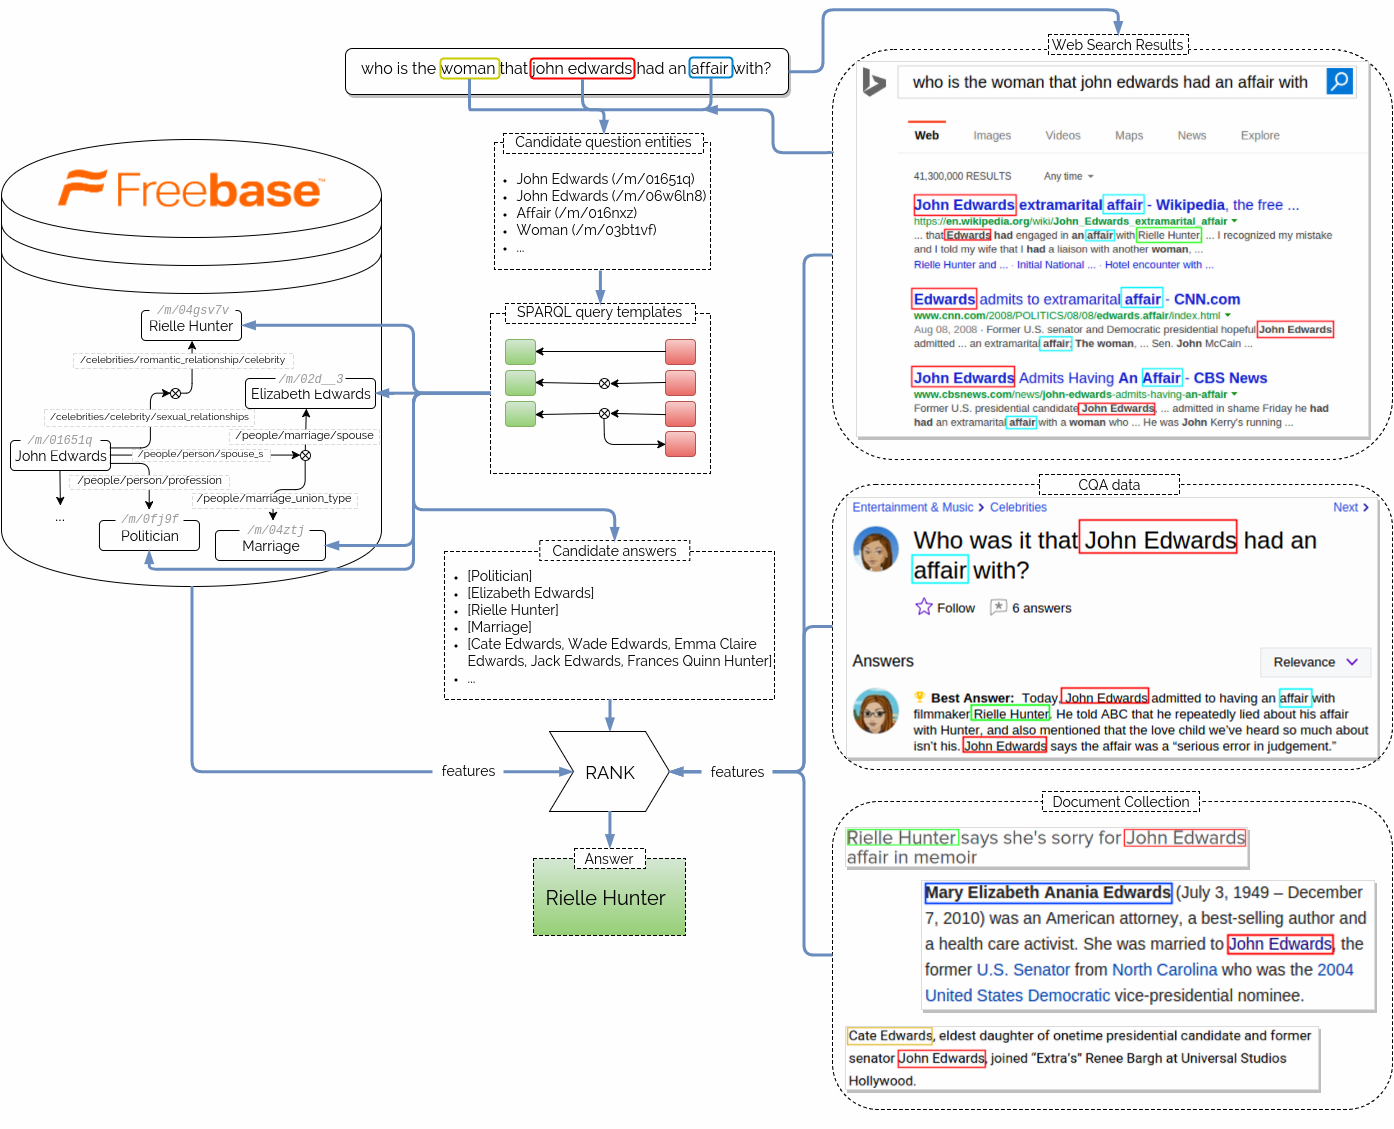
\includegraphics[width=1.0\textwidth]{img/Text2KB_model}
\caption{The architecture of our Text2KB Question Answering system}
\label{fig:text2kb:model}
\end{figure}

\subsubsection{Web search results for KBQA}
\label{subsubsec:text2kb:method:web}

To obtain related web search results, Text2KB issues the question as a query to a commercial web search engine\footnote{https://datamarket.azure.com/dataset/bing/search}, extracts top 10 search result snippets and the corresponding documents.
Next, it detects KB entity mentions in both snippets and documents.
% Document snippets are usually built to present the information most relevant to the query, and often contain answers to a question.
% Unfortunately, for longer queries the snippets often represent and combination of small phrases, that contain mostly question terms and very few additional information.
% Nevertheless, we keep both snippets and documents text, and using thesystem's linker detect KB entity mentions.
This data turns out to be useful for multiple purposes, \ie question entity identification and answer candidate ranking.

\textbf{Question entity identification}.
Question text provides only a limited context for entity disambiguation and linking; additionally, the entity name can be misspelled or an uncommon variation used.
This complicates the task of entity identification, which is the foundation of whole question answering process.
Fortunately, web search results help with these problems, as they usually contain multiple mentions of the same entities and provide more context for disambiguation.
Text2KB uses the search result snippets to {\em expand} the set of detected question entities.
To keep only the entities that are also mentioned in the question and avoid irrelevant entities, we use string distance.
More specifically, we take names of all entities detected in the question and compute their term by term similarity with non-stopwords from the question.
In this work we used Jaro-Winkler string distance and entity was added to the list of question entities if at least one of its tokens $e_t$ has high similarity with one of the question tokens $q_t$ excluding stopwords ($Stop$):
$$max_{e_t \in M\backslash Stop, q_t \in Q\backslash Stop} distance_{Jaro-Winkler}(e_t, q_t) \geq 0.8$$

\textbf{Answer candidate features}.
Most of the information stored in knowledge bases is also present in other formats, including natural language statements, tables, \etc
For example, on Figure \ref{fig:text2kb:web_search_entitylink} multiple snippets mention the date when Tutankhamun became the king.
Text-QA systems usually generate answer candidates from passages extracted from retrieved documents.
In our case candidates are already generated from a KB and we just need to rank them to select the best one.
Text2KB uses snippets and documents to compute a set of features, which are used for answer candidate ranking.
More specifically we do this following:

\begin{figure}[h]
\centering
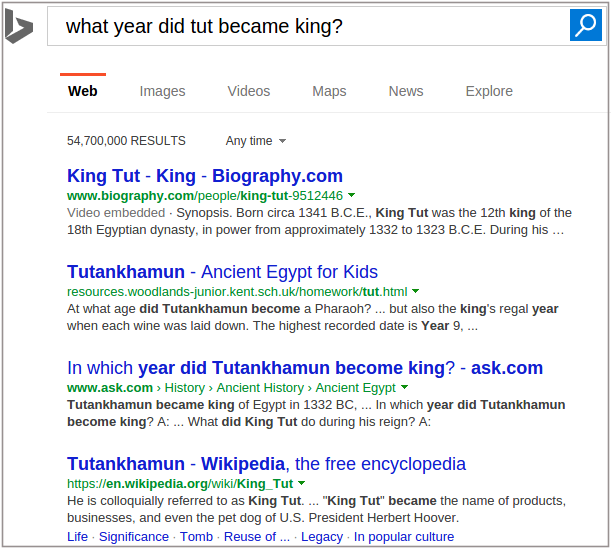
\includegraphics[width=0.5\textwidth]{img/web_search_entitylink}
\caption{Search results for the question \textit{``what year did tut became king?''}, which mention both the full name of the king and the correct answer to the question}
\label{fig:text2kb:web_search_entitylink}
\end{figure}

\begin{enumerate}
\setlength\itemsep{-0.5em}
\item Precompute term and entity IDFs\footnote{https://en.wikipedia.org/wiki/Tf-idf}. We used Google n-grams corpus to approximate terms IDF by collection frequencies and available ClueWeb Freebase entity annotations\footnote{http://lemurproject.org/clueweb09/FACC1/} to compute entity IDFs
\item Each snippet and document is represented by two TF-IDF vectors of lowercased tokens and mentioned entities
\item In addition, vectors of all snippets and all documents are merged together to form combined token and entity vectors
\item Each answer candidate is also represented as TF-IDF vectors of terms (from entity names) and entities
\item We compute cosine similarities between answer and each snippet and document token and entity vectors. This gives us 10 similarity scores for every document for token vectors and 10 similarities for entity vectors, we take average and maximum scores as features.
\item We do the same for the combined document and use cosine similarities as features.
\end{enumerate}

\subsubsection{CQA data for Matching Questions to Predicates}
\label{subsubsec:text2kb:method:cqa}

Recall that a major challenge in KBQA is that natural language questions do not easily or uniquely map to entities and predicates in a KB. An established approach for this task is supervised machine learning, which requires labeled examples of questions and the corresponding answer to learn this mapping. Unfortunately, manual labeling of questions with answers is expensive, and necessarily contains only a small fraction of the different ways the same KB predicate can be inquired about using natural language questions. Researchers have proposed to use weakly supervised methods to extend the lexicon with mappings learned from \textit{single sentence statements} mentioning entity pairs from a large corpus \cite{YaoD14}.
However, often there is a lexical gap between how information is asked about in a question and how it is expressed in a statement.
On the other hand there are huge archives of questions and answers posted by real users on various community question answering websites, \eg Figure \ref{fig:text2kb:cqa_example}.

\begin{figure}
\centering
\fbox{
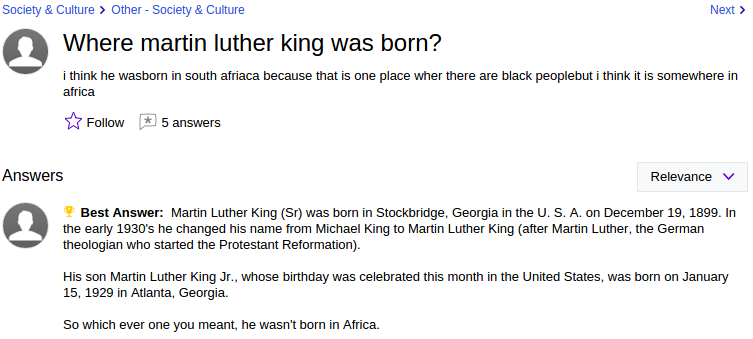
\includegraphics[width=0.5\textwidth]{img/cqa_example}
}
\caption{Example of a question and answer pair from Yahoo! Answers CQA website}
\label{fig:text2kb:cqa_example}
\end{figure}

For our experiments we use 4,483,032 questions from Yahoo! Comprehensive Questions and Answers WebScope dataset\footnote{https://webscope.sandbox.yahoo.com/catalog.php?datatype=l}.
Texts of each question and answer pair were run through an entity linker, that detected mentions of Freebase entities.
Next, similar to an idea of relation extraction from CQA data \cite{savenkov2015relation}, we use distant supervision to label each question-answer pair with predicates between entities mentioned in the question and in the answer.
As a result, we have a set of questions, annotated with KB predicates, which are, often incorrectly, assumed to answer the question.
We learn the associations between question terms and predicates by computing pointwise mutual information scores\footnote{https://en.wikipedia.org/wiki/Pointwise\_mutual\_information} (PMI) for each term-predicate pair.
Examples of scores for some terms from WebQuestions dataset questions are given in Table \ref{table:text2kb:cqa_npmi}.

\begin{table}
\centering
\caption{Examples of term-predicate pairs with high PMI scores, computed using distant supervision from a CQA collection}
\label{table:text2kb:cqa_npmi}
\begin{tabular}{| p{2cm} | p{8cm} | p{2cm} |}
\hline
Term & Predicate & PMI score\\
\hline
born & people.person.date\_of\_birth & 3.67\\
 & people.person.date\_of\_death & 2.73\\
 & location.location.people\_born\_here & 1.60\\
\hline
kill & people.deceased\_person.cause\_of\_death & 1.70\\
& book.book.characters & 1.55\\
\hline
currency & location.country.currency\_formerly\_used & 5.55 \\
& location.country.currency\_used & 3.54 \\
\hline
school & education.school.school\_district & 4.14 \\
& people.education.institution & 1.70\\
& sports.school\_sports\_team.school & 1.69 \\
\hline
illness & medicine.symptom.symptom\_of & 2.11\\
& medicine.decease.causes & 1.68\\
& medicine.disease.treatments & 1.59\\
\hline
win & sports.sports\_team.championships & 4.11\\
& sports.sports\_league.championship & 3.79\\
\hline
\end{tabular}
\end{table}

Although noisy, the statistics look reasonable to be used for candidate ranking.
In Text2KB we take candidate answer predicates and look up the  PMI scores between these predicates and terms in the question.
Missing pairs are given a score of 0, and minimum, average and maximum of these scores are used as features.
Since this kind of data is usually sparse, we also use pretrained word2vec word embeddings\footnote{https://code.google.com/p/word2vec/} to generate predicate embeddings by taking weighted average of term vectors from predicate's PMI table.
Each term's embedding vector is weighted by its PMI value (terms with negative score are skipped).
Then, we compute cosine similarities between predicate vector and question term vectors and take their minimum, average, maximum as features.
Similarity between the predicate vector and average question term vector is also computed.


\subsubsection{Estimating Entity Associations}
\label{subsubsec:text2kb:method:clueweb}

When ranking candidate answers, we are interested in estimating whether the entities in the question and the answer are related in a way asked in the question.
Existing systems usually look on how candidate predicates are expressed in questions and statements.
But predicate isn't the only way we can look at this. An alternative is to consider text passages, \eg sentences, that mention topical and answer entities together.
For example, in the bottom right corner of Figure \ref{fig:text2kb:model} we can see some passages that mentioned a pair of people, and the context of these mentions often expresses the nature of the relationships between the entities.

We use the ClueWeb12 corpus with existing Freebase entity annotations\footnote{http://lemurproject.org/clueweb12/FACC1/} and compute counts of different terms that occur in the context to an entity pair mention.
By an entity pair mention we mean a pair of mentions of different entities within 200 characters of each other.
We take terms in between mentions and 100 character before and after mentions as the context.
A small sample of this data is presented in Table \ref{table:text2kb:clueweb_entitypairs_langmodel}.

\begin{table}
\centering
\caption{Example of entity pairs along with the most popular terms mentioned around the entities}
\label{table:text2kb:clueweb_entitypairs_langmodel}
\begin{tabular}{| p{4cm} | p{4cm} | p{8cm} |}
\hline
Entity 1 & Entity 2 & Term counts\\
\hline
John Edwards & Rielle Hunter & campaign, affair, mistress, child, former ...\\
\hline
John Edwards & Cate Edwards & daughter, former, senator, courthouse, left, greensboro, eldest ...\\
\hline
John Edwards & Elizabeth Edwards & wife, hunter, campaign, affair, cancer, rielle, husband ...\\
\hline
John Edwards & Frances Quinn Hunter & daughter, john, rielle, father, child, former, paternity...\\
\hline
\end{tabular}
\end{table}

First, given a set of question terms $Q$ and an answer candidate, that starts from a question entity $e_1$, we compute a language model score for every answer entity $e_2$:
$$p(Q|e_1, e_2) = \prod_{t\in Q} p(t | e_1, e_2)$$
and use minimum, average and maximum as features.
To address the sparsity problem, we again use embeddings, 
ie for each entity pair a weighted (by counts) average embedding vector of terms is computed and minimum, average and maximum cosine similarities between these vectors and question tokens vector are used as features.

\subsubsection{Internal text data to enrich entity representation}
\label{subsubsec:text2kb:internal_text}

In addition to external text data, many knowledge bases, including Freebase, contain text data as well.
In Freebase, most of the entities contain a description paragraph, which often comes from the entity Wikipedia profile.
These descriptions of entities in the KB were found useful for text-based question answering \cite{Sun:2015:ODQ:2736277.2741651}.
For completeness, we include them in our system. The aim is to improve the matching of the question text, to the unstructured description of the candidate entities. For this, each entity description is represented as a vector of tokens, and a vector of mentioned entities. We compute cosine similarities between the question tokens and each of the candidate entity vectors, and use these scores as features for candidate ranking.
In future work, we could explore incorporating any other entity profile text, such as full Wikipedia article.


\subsubsection{Evaluation}
\label{subsubsec:text2kb:evaluation}

We followed the standard evaluation procedure for the WebQuestions dataset and used the original 70-30\% train-test split, which results in 3,778 training and 2,032 test questions.
Since each answer is potentially a list of entities $a^*$, the quality of an answer $a$ is represented by F1-score: 
$$f1(a^*, a) = 2\frac{precision(a^*,a) recall(a^*,a)}{precision(a^*,a) + recall(a^*,a)}$$
where $precision(a^*, a)=\frac{|a^* \cap a|}{|a|}$ and $recall(a^*, a) = \frac{|a^* \cap a|}{|a^*|}$.

We also report average precision and recall, as well as an F1 score of average precision and recall.
The results of existing approaches, our baseline and Text2KB systems is presented in Table \ref{table:text2kb:webquestions_results}.

\begin{table}
\centering
\caption{Performance of the Text2KB system on WebQuestions dataset compared to the existing approaches. The difference from the baseline Aqqu system is significant with p-value < 0.01}
\label{table:text2kb:webquestions_results}
\begin{tabular}{| p{5cm} | p{1.5cm} | p{1.5cm} | p{1.5cm} | p{1.5cm} | }
\hline
System & avg Recall & avg Precision & F1 of avg Prec and Recall & avg F1 \\
\hline
SemPre \cite{BerantCFL13:sempre} & 0.413 & 0.480 & 0.444 & 0.357\\
Subgraph Embeddings \cite{BordesCW14:emnlp} & - & - & 0.432 & 0.392\\
ParaSemPre \cite{BerantL14:parasempre} & 0.466 & 0.405 & 0.433 & 0.399\\
Jacana \cite{YaoD14} & 0.458 & 0.517 & 0.486 & 0.330\\
Kitt AI \cite{yao-scratch-qa-naacl2015} & 0.545 & 0.526 & 0.535 & 0.443\\
AgendaIL \cite{berant2015imitation} & 0.557 & 0.505 & 0.530 & 0.497\\
STAGG \cite{yih:ACL:2015:STAGG} & \textbf{0.607} & \textbf{0.528} & \textbf{0.565} & \textbf{0.525}\\
% STAGG (no duplicates\footnote{An answer of the STAGG system may contain duplicate entities, which are double counted by the evaluation script}) \cite{yih2015semantic} & 0.6067 & 0.5263 & 0.5634 & 0.5234 \\
\hline
Aqqu (baseline) \cite{bastmore:cikm:2015:aquu} & 0.604 & 0.498 & 0.546 & 0.494\\
% DIDN'T HAVE TIME TO IMPLEMENT THIS.
% Text-only baseline & & & & \\
Our system: Text2KB & 0.6354 & 0.5059 & 0.5633 & 0.5223 \\
\hline
\end{tabular}
\end{table}

As we can see, Text2KB significantly improves over the baseline system and reaches the current best published result - STAGG \cite{yih:ACL:2015:STAGG}, and we believe that this system will also benefit from the ideas of our work, and we will explore this question in Section \ref{section:text2kb:analysis}.

\textbf{Ablation Study}.
To study effects of different components in isolation we made a series of ablation studies.
For convenience, we introduce the following notations for different components of our system:
\begin{itemize}
\setlength\itemsep{-0.5em}
\item T - notable type score model as a ranking feature
\item DF - date range filter-based query template
% \item TF - using notable type based filter
\item E - using web search result snippets for question entity identification
\item W - using web search results for feature generation
\item CQA - using CQA-based \texttt{[question term, KB predicate]} PMI scores for feature generation
\item CW - features, computed from entity pairs language model, estimated on ClueWeb
\end{itemize}

In our results table we will use the notation \texttt{+$<$component$>$} to for a system with a certain component added, and \texttt{-$<$component$>$} when the component is removed.
For example, the baseline system will be denoted as ``\texttt{Aqqu}'' according the authors notation.
The same system with additional date range filter query templates and notable types score model is denoted as ``\texttt{Aqqu +DF+T}'', which represents the same system as ``\texttt{Text2KB -E-W-CQA-CL}''.
Our full system ``\texttt{Text2KB}'' can be also denoted as ``\texttt{Aqqu +DF+T+E+W+CQA+CL}''.

\begin{table}
\centering
\caption{Average Recall (R), Precision (Pr), and F1 of Aqqu (baseline), Text2KB (our system), and variations of TextKB with respective components removed. * indicates significant differences at p<0.05. }
\label{table:text2kb:ablation:entities_vs_features}
\begin{tabular}{| p{7cm} | c | c | c | }
\hline
System & R & Pr & F1 \\
\hline
% THIS TELLS HOW MUCH EXTERNAL ENTITIES GIVE COMPARED TO MY OTHER IMPROVEMENTS
\texttt{Aqqu} (baseline) & 0.604 & 0.498 & 0.494\\
% baseline_typemodel_dates.log : baseline with types model +dates, but without any text-based data
\texttt{Text2KB -E-W-CQA-CL}=\texttt{Aqqu +DF+T} & 0.6169 & 0.4807 & 0.4987 \\
% extent_dates_typemodel_rf100.log : -web-cqa-clueweb
\texttt{Text2KB -W-CQA-CL} & 0.6272* & 0.4920* & 0.5083* \\  % AND FEATURES GIVE THE REST
% web_cqa_clueweb_typemodel_dates.log : -external entities (Text features on top my other improvements)
\texttt{Text2KB -E} & 0.6344* & 0.4966* & 0.5140* \\  % AND FEATURES GIVE THE REST
%\hline
% extent_web_cqa_clueweb_dates_types_typemodel_rf100.log : everything, including type filters
%\texttt{Text2KB} & 0.6354* & 0.5059* & 0.5223* \\
\hline
\end{tabular}
\end{table}

The first question that we are asking is what are the improvements, introduced by adding date range filter templates, notable type model, entity linking from web search results and text-based features generated from all the different sources.
Results of this ablation experiment are presented in Table \ref{table:text2kb:ablation:entities_vs_features}.
As we can see, additional date range filters and notable types model (\texttt{Text2KB -E-W-CQA-CL}) are responsible for an increased recall and a drop in precision compared to the baseline model.
Detecting question entities (\texttt{Text2KB -W-CQA-CL}) help improve both precision and recall, and therefore average F1 score by 0.096 points.
An even bigger improvement is achieved by introducing all our external text-based features, and since these improvements are independent, their combination boosts the performance even more.

Now, let's look into the relative importance of each of the data sources, we will remove or use a group of web search, cqa or clueweb-based features and see how the performance of the whole system changes.
Table \ref{table:text2kb:ablation:features} summarizes the results of these experiments.

\begin{table}
\centering
\caption{Average Recall (R), Precision (Pr), and F1 of Text2KB variations with and without features based on web search results, CQA data and ClueWeb collection}
\label{table:text2kb:ablation:features}
\begin{tabular}{| p{7cm} | c | c | c | }
\hline
System & R & Pr &  F1 \\
\hline
% THIS PART ANSWERS HOW GOOD ARE EACH OF THE PROPOSED DATASETS
% extent_cqa_clueweb_dates_typemodel_rf100.log : -web
\texttt{Text2KB -W} & 0.6327 & 0.4960 & 0.5126 \\
% extent_web_clueweb_dates_typemodel_rf100.log : -cqa
\texttt{Text2KB -CQA} & 0.6420 & 0.4987 & 0.5185 \\
% extent_web_cqa_dates_typemodel_rf100.log : -clueweb
\texttt{Text2KB -CL} & 0.6444 & 0.5047 & 0.5228 \\
\hline
% extent_web_dates_typemodel_rf100.log : -clueweb-cqa
\texttt{Text2KB} (Web search results only) & 0.6423 & 0.5028 & 0.5216 \\
% extent_clue_dates_typemodel_rf100.log : -web-cqa
\texttt{Text2KB} (ClueWeb only) & 0.6307 & 0.4978 & 0.5138 \\
% extent_cqa_dates_typemodel_rf100.log : -web-clueweb
\texttt{Text2KB} (CQA only) & 0.6224 & 0.4928 & 0.5077 \\
%\hline
% extent_web_cqa_clueweb_dates_types_typemodel_rf100.log : everything, including type filters
%\texttt{Text2KB} & 0.6354 & 0.5059 & 0.5223 \\
\hline
\end{tabular}
\end{table}

Features that we generate from web search results are the most effective, because even without other data sources the QA performance is almost as high as the full system.
In addition, if we remove web search results based features the performance drops more than for other text data sources.
Features based on ClueWeb entity pair statistics perform better than CQA-based features.

% THIS EXPERIMENTS ARE REDUNDANT
%\begin{table}
%\caption{Evaluation study for our system with different text-based data sources used to generate features}
%\label{table:ablation:other}
%\begin{tabular}{| p{4cm} | c | c | c | }
%\hline
%System & avg Re & avg Pr &  avg F1 \\
%\hline
%AQQU & 0.604 & 0.498 & 0.494\\
%Text2KB -TF & 0.6429 & 0.5030 & 0.5220 \\
%\hline
% THIS PART SHOULD ANSWER HOW TEXT BASED FEATURED COMPARE TO EXTERNAL ENTITIES
% web_cqa_clueweb_typemodel_rf100.log : web+cqa+clueweb+typemodel -external-dates
%Text2KB +W+CQA+CW+T-E & 0.6351 & 0.4933 & 0.5104 \\
% web_cqa_clueweb_noext_rf100.log : web+cqa+clueweb -external-dates-typemodel
%Text2KB +W+CQA+CW-E & 0.6414 & 0.4981 & 0.5160 \\
% typemodel_rf100.log : type model only
%Text2KB +T-W-CQA-CL-E & 0.6131 & 0.4747 & 0.4918 \\
%\hline
%\end{tabular}
%\end{table}

Since we used each data source to generate multiple different features for candidate ranking, it is interesting to see which particular features are  more useful than others by the ranking machine learning algorithm (we used random forest).
Figure \ref{fig:text2kb:feature_importances} plots a subset of features ranked by their Gini index-based importance scores in the final answer candidate ranking model.

\begin{figure}
\centering
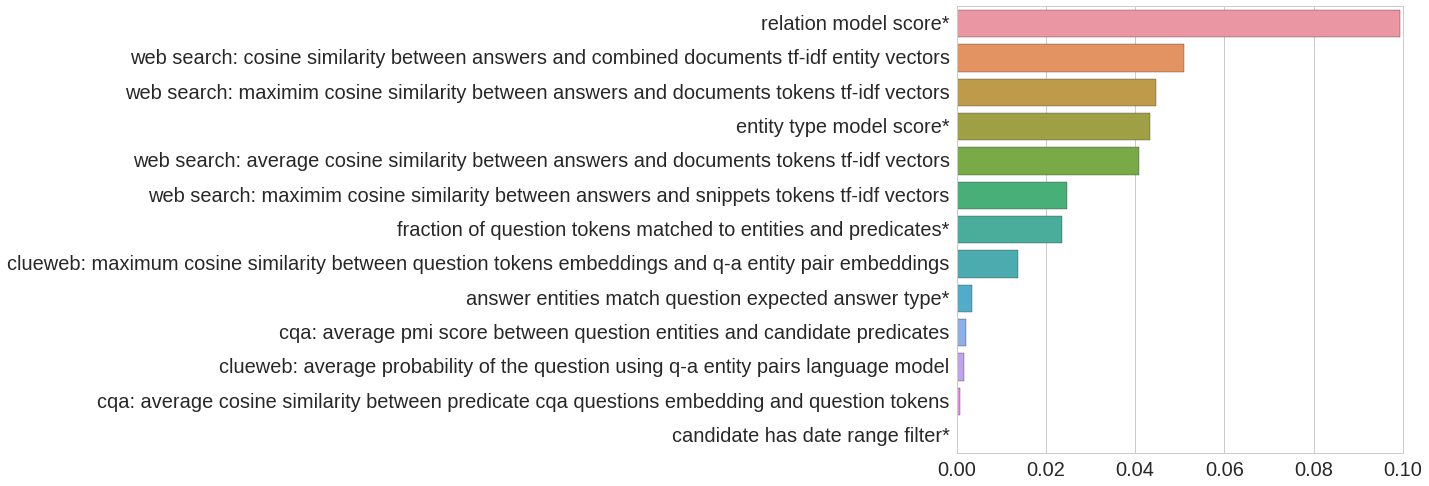
\includegraphics[width=0.9\textwidth]{img/feature_importances}
\caption{Importances of different text-based features for KBQA (features with * are not text-based and are provided for comparison)}
\label{fig:text2kb:feature_importances}
\end{figure}

The figure supports the observation that web search results features are the most useful, however, other text data sources also contribute to the improvement.

In summary, Text2KB significantly outperforms the baseline system, and each of the introduced components contributes to this improvement.
Web search results data turned out to be the most useful resource, and it significantly improves the quality by helping with question entity identification and candidate ranking.
Next, we analyze the system performance in more detail, and investigate factors for future extension.

\subsubsection{Analysis}
\label{subsubsec:text2kb:analysis}

We have shown that Text2KB outperforms the baseline.
We now investigate how our system would compare to other systems on the same benchmark; then, we investigate in depth the different error modes, which helps identify the areas of most substantial future improvements. 

% Don't have a better name for now. By generalization I mean whether our results are system specific or universally useful.
% \subsection{Generalization analysis}


\begin{table}
\centering
\caption{Average Recall (R), Precision (Pr), and F1 for Text2KB (our system), STAGG and their combinations}
\label{table:text2kb:combine_stagg}
\begin{tabular}{| p{4cm} | p{1cm} | p{1cm} | p{1cm} | }
\hline
System & R & P & F1 \\
\hline
%Aqqu (baseline) \cite{ACCU:2015} & 0.604 & 0.498 & 0.494\\
% DIDN'T HAVE TIME TO IMPLEMENT THIS.
% Text-only baseline & & & & \\
Our system: Text2KB & 0.6354 & 0.5059 & 0.5223 \\
STAGG \cite{yih:ACL:2015:STAGG} & 0.607 & 0.528 & 0.525\\
\hline
Text2KB + STAGG & 0.5976 & 0.5343 & 0.5320 \\
Text2KB + STAGG (oracle) & 0.7144 & 0.5904 & 0.6056 \\
\hline
\end{tabular}
\end{table}

We took an existing KBQA systems and demonstrated that by combining evidence from knowledge base and external text resources we can boost the performance.
A reasonable question is whether the same approach will be helpful to other systems, \eg the currently best system STAGG \cite{yih:ACL:2015:STAGG}.
The differences between our baseline system Aqqu and STAGG lie in the components, \ie entity linking algorithm, a set of query templates and ranking methods, therefore our approach is complementary and should be helpful.
To support this claim, we made an experiment to combine answers of STAGG and Text2KB.
One of the advantages of the former is its set of filters, that restricts list results to entities of certain type, gender, \etc
Therefore, we combined answers of STAGG and Text2KB using a simple heuristic: we chose to use the answer returned by STAGG if the number of answer entities is less than in the Text2KB answer, otherwise we use the answer of our approach.
Table \ref{table:text2kb:combine_stagg} gives the results of the experiment, and as we can see the combination achieves slightly better average F1 score.
Alternatively, we can look at the oracle combination of the systems, which always chooses an answer with higher F1.
This experiment shows that that systems don't make exactly the same mistakes and therefore can be combined.
As we can see such a combination results in a performance of 0.6056, which is much higher than either of the systems.

WebQuestions dataset is rather small as a result, answers to 112 of the test questions involve a predicate that weren't observed in the training set, which may be a problem for approaches that rely on a trained lexicon.
We evaluated both systems on these questions, and indeed the performance is very low, \ie the average F1 score of Text2KB is 0.1640 compared to 0.1199 for STAGG\footnote{Unfortunately, the number of questions is too low to show statistical significance (p-value=0.16)}.

\begin{figure}
\centering
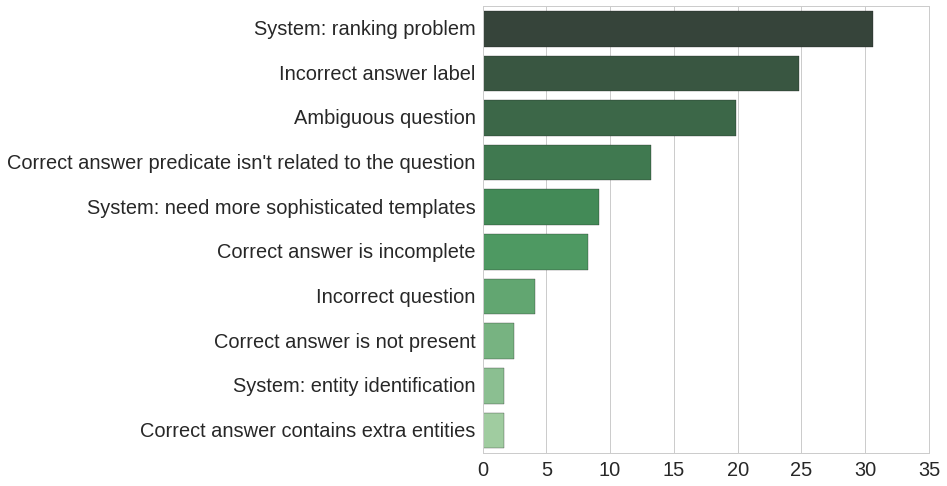
\includegraphics[width=0.45\textwidth]{img/error_analysis}
\caption{Distribution of problems with questions, where Text2KB returns an answer with F1$<$1}
\label{fig:text2kb:error_analysis}
\end{figure}

To get a better insights of the problems that remain, we collected 1219 questions for which Text2KB didn't return completely correct answer, \ie F1 score of the answer is less than 1.
We manually looked through a couple of hundreds of these examples and grouped the problems into several clusters.
The results are summarized on Figure \ref{fig:text2kb:error_analysis}.

As we can see candidate ranking is still the major problem, and it accounts for $~31\%$ of the cases.
The second most popular problem is incorrect ground truth labels (almost a quarter of errors).
For example: for the question \textit{when tupac was shot?''} the label says \texttt{Tupac 1994 assault} instead of \texttt{Las Vegas}.
Another set of questions have incomplete or overcomplete ground truth answer list.
Typical examples are questions asking for a list of movies, books, landmarks, \etc
The ground truth answer usually contains $\sim10$ entities, whereas the full list is often much larger.
This seems to be an artifact of the labeling process, where the answer was selected from the Freebase entity profile page.
The profile page shows only a sample of 10 entities from large lists and the others are hidden behind the ``NNN values total'' link.
About 20\% of the questions are ambiguous, \ie questions have no strict 1-1 correspondence with any of the predicates and can be answered by multiple without any obvious preferences.
% for the question \textit{``where is shakira from?''} the ground truth is the country - \texttt{Colombia}, while Text2KB returned her place of birth - \texttt{Barranquilla}.
For example, the question \textit{``what did hayes do?''} can be answered by profession, occupied position or some other achievements.
Another problem is when there is no predicate that answers the question.
For example, the question \textit{``what do people in france like to do for fun?''} doesn't have a good match among the facts stored in Freebase.
The ground truth entity \texttt{Cycling} comes from predicate related to the olympic sport competitions country participated in\footnote{\texttt{olympics.olympic\_participating\_country.athletes}}, which obviously isn't related to the question.
% In some cases there are entities that are very similar in meaning, but represented in Freebase by different ids and names.
% For example, the answer to the question \textit{``what is william taft famous for?''} is \textit{``President of the United States''}, which is a government position, but there is also a triple \texttt{[William Howard Taft, common.topic.notable\_for, US President]}, where the last entity represents a type of people who help the position, and is considered incorrect.

% This is nice, but probably is too little to mention.
% We also noticed, that in a small number of examples, the case of the correct answer entity and the answer returned by the system is different.
% For example, for the question \textit{``what fma stands for?''} the correct answer specified in the dataset is \textit{``FullMetal Alchemist''}, while the actual name of the entity is \textit{``Fullmetal Alchemist''}.
% The official evaluation script don't normalize the case and therefore considers this example incorrect.
% If we lowercase all entity names before comparison, the average F1 score of Text2KB becomes 0.5248.

As for the system errors, there are wins and loses introduced by each of our components.
Web search results helped identify the right question topical entity in a number of cases, \eg \textit{``what did romo do?''} mentions only the last name of the Dallas Cowboys quarterback and the baseline system were unable to map it to the right entity.
Web search results provides more than enough evidence that romo refers to \texttt{Tomo Romo}.
However, there are a number of loses, introduced by added unrelated entities.
For example, the entity \texttt{I Love Lucy} was added for the question \textit{``what was lucille ball?''}, because the term \textit{lucy} had high similarity with \textit{lucille}.
A portion of these problems can be fixed by a better entity linking strategy, \eg \cite{SMAPH_ERD:2014}.

% For the question \textit{``what did bruce jenner win gold medal for?''} the baseline system answered \textit{``1976 Summer Olympics''}, but web search results mention decathlon many times and thus Text2KB was able to rerank the candidates and return the entity \textit{``Athletics at the 1976 Summer Olympics - Men's Decathlon''}\footnote{Unfortunately, the entity selected as the answer during labeling is \textit{``Decathlon Challenge''}, which is a book Bruce Jenner wrote}.

An interesting example, when external text resources improved the performance is the question \textit{``what ship did darwin sail around the world?''}.
This is actually a hard question, because the ship entity is connected to the \texttt{Charles Darwin} entity through the ``knownFor'' predicate along with some other entities like \texttt{Natural selection}.
% \footnote{\texttt{user.lindenb.default\_domain.scientist.known\_for}
Thus, the predicate itself isn't related to the question, but nevertheless, the name of the ship \texttt{HMS Beagle} is mentioned multiple times in the web search results, and entity pair model computed from ClueWeb also has high scores for the terms ``ship'' and ``world''.

There are several major reasons for the loses, introduced by features based on external text resources.
Some entities often mentioned together and therefore one of them gets high values of cooccurrence features.
For example, the baseline system answered the question \textit{``when did tony romo got drafted?''} correctly, but since \texttt{Tony Romo} is often followed by \texttt{Dallas Cowboys}, Text2KB ranked the team name higher.
Another common problem with our features is an artifact of entity linking, which works better for names and often skips abstract entities, like professions.
For example, the correct answer to the question \textit{``what did jesse owens won?''} is an entity with the name \texttt{Associated Press Male Athlete of the Year}, which is rarely mentioned or it's hard to find such mentions.
Some problems were introduced by a combination of components.
For example, for \textit{``where buddha come from?''} a topical entity \texttt{Buddhism} was introduced from search results, and it generated \texttt{Gautama Buddha} as one of the answer candidates.
This answer was ranked the highest due to large number of mentions in the search results.
% In some cases search results aren't very relevant and only provide general information about question entity.

% Also problems of the original system persist, especially problems with the relation score model and popular predicates.

% I already mentioned this...
% WebQuestions dataset isn't free of noise and quite a few answers are actually incorrect for various reasons.
% When labeling the question ``what team does jordan own?'' mechanical turk workers had to select the answer from the page, corresponding to the country and not \textit{Michael Jordan} the basketball player.


% Non-relevant
% The first set of improvements come from the date range filter template, \eg for the question \textit{``who is the current leader of france 2010?''} our system returns a single correct result \textit{``Nicolas Sarkozy''} instead of the list of all French presidents.
% The type model score feature helped in some cases, where there is a clear indication of the type of entity, expected as the answer, \eg \textit{``which state did anne hutchinson found?''} - \textit{``Rhode Island''}.

In summary, we show that ideas behind Text2KB could be integrated into other systems and improve their performance.
The error analysis suggested that even though a significant number of questions in the WebQuestions dataset have incorrect or ambiguous ground truth labels, there is still a room for improvement.
In particular, the future work for Text2KB will include a better strategy for entity linking using external data sources and a better context model for entity mentions in text documents, which can put more weight on entities mentioned in the context related to the question.

\subsubsection{Conclusion}
\label{subsubsec:text2kb:conclusion}

Our work showed that unstructured text resources can be effectively utilized for knowledge base question answering to improve query understanding,  candidate answer generation and ranking.
We focused on three particular techniques and associated text information sources: web search results for query understanding and candidate ranking, community question answering data for candidate generation, and text fragments around entity pair mentions for ranking. Certainly, there are more resources that could be potential adapted, \eg entity profile pages like Wikipedia, news sources, textbooks, and many others. However, we believe that the proposed approach is general enough that it could be extended and successfully incorporate these other diverse text sources.

In the future, we plan to extend our work to the more open setup, similar to the QALD hybrid task, where questions no longer have to be answered exclusively from the KB. This would require extending the described techniques, and creating new QA benchmarks.



\subsection{Hybrid Question Answering over Knowledge Bases and Semantically Annotated Text Collections}
\label{subsec:text+kb}

\begin{figure*}
\centering
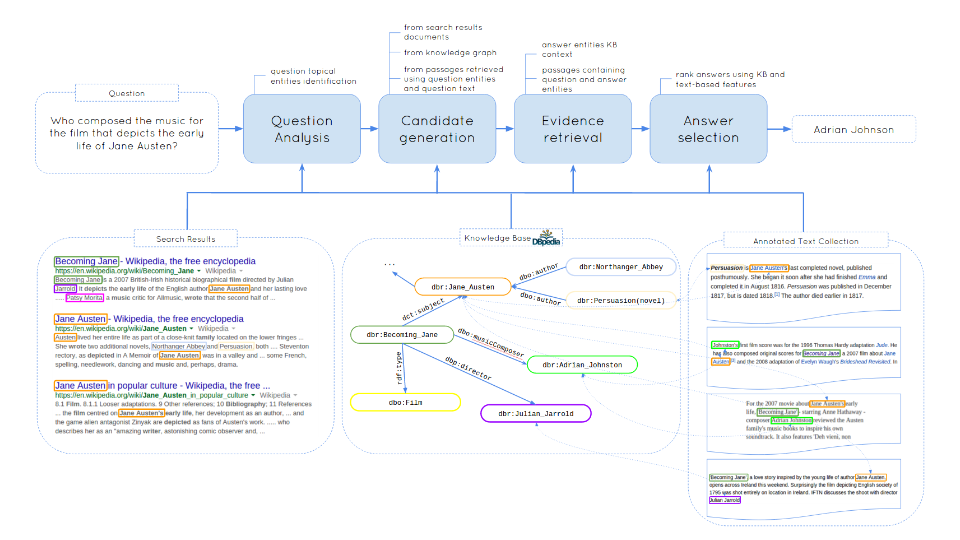
\includegraphics[width=\textwidth]{img/text_and_kb}
\caption{Architecture of a hybrid factoid question answering system, that uses a combination of structured knowledge base and unstructured text data}
\label{fig:text_kb}
\end{figure*}

The architecture of the hybrid QA model I propose is presented on Figure \ref{fig:text_kb}.
Here are the main stages of the question answering process:
\begin{itemize}
\setlength\itemsep{0em}
\item \textbf{Pre-processing}: identify mentions of KB entities in text document collection and index the documents text and mentions in separate fields
\item \textbf{Topical entity identification}: search the text collection using question (or reformulated question \cite{AgichteinLG01}) as a query and use an approach similar to \cite{cornolti2014smaph} to detect question topical entities
\item \textbf{Candidate generation from text}: extract candidate answer (or intermediate answer) entities with evidence from the retrieved text documents using existing techniques, e.g. \cite{tsai2015web}.
\item \textbf{Candidate generation from KB}: explore the KB neighborhood of question topical entities and entities extracted from text documents on the previous step
\item \textbf{Candidate generation from KB \& Text}: use entity and text index to find entities mentioned near question topical entity and question terms in the document collection
\item \textbf{KB evidence extraction}: match neighborhood of answer entities (entity type and other entities) against the question to get additional evidence
\item \textbf{Text evidence extraction}: estimate the similarity between the collection text fragments mentioning question and answer entities and the question text
\item \textbf{Rank candidate}: rank candidate answers using evidence extracted from the KB as well as from text
\end{itemize}

Let's consider an example question ``\textit{Who composed the music for the film that depicted the early life of Jane Austen?}'' from the QALD dataset\footnote{http://greententacle.techfak.uni-bielefeld.de/~cunger/qald/} (Figure \ref{fig:text_kb}).
Even though it's quite easy to identify the ``\texttt{Jane Austen}'' entity in the question, the knowledge base (dbPedia in this example) cannot help us to determine which movie is being referred to.
However, there are a lot of documents on the web, that do mention the ``\texttt{Becoming Jane}'' movie and say what is it about.
Unfortunately, extracting the name of the composer from these documents is quite challenging, but this task can be easily accomplished by checking the value of the \texttt{musicComposer} property in the knowledge base.
At the end, for each candidate answer entity, we have all the KB information and passages that mention this entity as evidence to help with the correct answer selection.

\subsubsection{Evaluation}
\label{sec:factoid_evaluation}


I THINK HERE WE CAN INCLUDE OUR RESULTS ON TEXT2KB.

Most of the recent work on knowledge base question answering and semantic parsing have been evaluated on the WebQuestions dataset \cite{BerantCFL13:sempre}, which contains a collection of question text and correct answer entities.
The questions were collected using Google Suggest API and answers crowdsourced using Amazon Mechanical Turk\footnote{http://mturk.com/}
The proposed approach will be compared against the previous results\footnote{http://goo.gl/sePBja} on this dataset.
Again, web can be used as a text collection which can be queried using Bing Search API.
Relation extraction patterns can be mined using distant supervision from ClueWeb collection using publicly available dataset of Freebase annotations \cite{gabrilovich2013facc1}.

\textbf{New factoid question answering dataset}.
However, WebQuestions dataset has certain limitations, e.g. questions mined using Google Suggest API have very similar structure and lexicon, and to find the answer to the mined questions users were asked to use the question entity Freebase profile page,  which only include entities connected directly with a predicate or through a mediator node.
Therefore most of the state-of-the-art results on the dataset use a small number of predefined logical form patterns.
On the other hand CQA websites have a fraction of factoid questions with provided text answers.
Here I propose to use to construct a new dataset for question answering over Freebase by selecting a subset of QnA pairs with at least one entity in question and answer and some reasonable filtering heuristics and manual validation using crowdsourcing (e.g. through Amazon Mechanical Turk).
Existing systems need to be retrained and tested on the new dataset to compare against the proposed model.

...........

TREC QA datasets served as a benchmark for various question answering systems.
Therefore, to evaluate the proposed approach for question answering over text enriched with the structured data I propose to test it on dataset derived from TREC QA and compare against existing strong baselines, including the most related approaches \cite{Fader:2014:OQA:2623330.2623677,Sun:2015:ODQ:2736277.2741651}.
The proposed system can use the web as the corpus and query it using Bing Search API\footnote{https://datamarket.azure.com/dataset/bing/searchweb}.
Freebase and Reverb extractions \cite{FaderSE11} are examples of schema-based and open knowledge bases that can be used for the experiments.
The metrics used for evaluation typically include accuracy and mean reciprocal rank (MRR).

For non-factoid question answering this year TREC pioneered a new question answering track - TREC LiveQA\footnote{http://trec-liveqa.org/}, which targets questions asked by real users of Yahoo! Answers website.
This year the deadline for system submission was on August 31 and my system trained on CQA QnA pairs participated in the challenge.
The results will be available on the TREC Conference in November 2015.
Organizers plan to continue with another TREC LiveQA task next year and this is going to be a good estimation of the effectiveness of the proposed techniques on hard real user questions.


\section{Summary}
In this section we considered two different ways of combining unstructured and structured data to improve factoid question answering.
Relation extraction from question-answer pairs aims at filling some gaps in KB fact coverage, whereas semantic annotations of text documents provides a way to incorporate information available in unstructured text documents for reasoning along with KB data to improve the performance of factoid question answering.

Factoid questions represent just a part of user information needs. Many problems require more elaborate response, such as a sentence, list of instructions or in general a passage of text.
Such questions are usually referred to as non-factoid questions and they will be the focus of the next Chapter.

\clearpage

%--- THE NEXT PIECE IS OLDER, NEED TO REVIEW

%Question answering from text corpora typically starts by retrieving a set of potentially relevant documents using the question (or some transformation of the question \cite{AgichteinLG01}) as the query, and then extracting entities, phrases, sentences or paragraphs believed to be the answer to the question.
%However, the information available in the retrieved pieces of text is very limited and often not enough to decide whether it can be the answer to the given question.
%For example, below is one of the questions from TREC QA 2007 dataset:\\
%\textit{``What republican senators supported the nomination of Harriet Miers to the Supreme Court?''}\\
%A candidate answer sentence \textit{``Minority Leader Harry Reid had already offered his open support for Miers.''} mentions a senator ``Harry Reid'' and clearly says about his support of the nomination.
%However, ``Harry Reid'' is not a correct answer to the question because he is a member of the Democratic party.
%This information is not available in the answer candidate sentence, but it is present as one of the properties in Freebase: [Harry Reid, political\_party, Democratic party]\footnote{Actually, in Freebase the entities are connected by a path of length 2 through a mediator node. The predicates on the path are: /government/politician/party and /government/political\_party\_tenure/party}.
%Therefore, by looking into the knowledge available about the mentioned entities a QA system can make a better judgment about the candidate answer.

% THIS IS THE CORRESPONDING PIECE ON KBQA, I DON'T REALLY LIKE IT

% Question answering over linked data (knowledge bases) converts a natural language question into a structured query, such as SPARQL.
%The main challenge for such systems is to map words and phrases from the question to the corresponding entities and predicates from a KB.
%Usually, such lexicon is built during training using ground truth question-query pairs \cite{CaiY13} or question-answer pairs \cite{BerantCFL13:sempre}.
%Improvements were made by extending the lexicon using Wikipedia and patterns expressing certain predicates obtained via distant supervision \cite{bastmore:cikm:2015:aquu,BordesCW14:emnlp,ReddyLS14,yih:ACL:2015:STAGG,YaoD14}.
%But still, the amount of available labeled or weakly labeled training data is much smaller than the amount of unstructured data.
%This unstructured data will complement the learned lexicon, e.g. even if a question about a certain predicate wasn't seen during training, a set of text paragraphs mentioning both of the related entities can provide a QA system with enough evidence to make the correct decision.
